\documentclass[11pt]{article}

\usepackage[T1]{fontenc}
\usepackage[utf8]{inputenc}
\usepackage{lmodern}
\usepackage{microtype}
\usepackage[margin=0.82in]{geometry}
\usepackage{amsmath,amssymb,mathtools}
\usepackage{booktabs}
\usepackage{array}
\usepackage{enumitem}
\usepackage[most]{tcolorbox}
\usepackage{tikz}
\usetikzlibrary{arrows.meta,calc,decorations.pathreplacing,positioning,angles,quotes}
\usepackage{fancyhdr}
\usepackage{hyperref}
\usepackage{needspace}
\usepackage{graphicx}

\hypersetup{
  colorlinks=true,
  linkcolor=blue!55!black,
  urlcolor=blue!55!black,
  pdftitle={Exercise 8.6: The Method of Halves and Viete's Product},
  pdfauthor={OpenAI}
}

\setlength{\parindent}{0pt}
\setlength{\parskip}{0.62em}
\setlist[itemize]{leftmargin=1.55em,itemsep=0.25em,topsep=0.25em}
\setlist[enumerate]{leftmargin=1.75em,itemsep=0.35em,topsep=0.3em}
\allowdisplaybreaks
\setcounter{tocdepth}{1}

\pagestyle{fancy}
\fancyhf{}
\lhead{Exercise 8.6 Tutorial}
\rhead{The Method of Halves}
\cfoot{\thepage}
\setlength{\headheight}{14pt}

\definecolor{navy}{RGB}{24,55,93}
\definecolor{softblue}{RGB}{235,244,252}
\definecolor{softgreen}{RGB}{236,248,239}
\definecolor{softyellow}{RGB}{255,249,226}
\definecolor{softred}{RGB}{253,239,239}
\definecolor{softgray}{RGB}{245,246,248}

\newtcolorbox{problemBox}{
  enhanced,
  colback=softblue,
  colframe=navy,
  boxrule=0.8pt,
  arc=2mm,
  title=The problem,
  fonttitle=\bfseries,
  breakable
}

\newtcolorbox{ideaBox}[1][Key idea]{
  enhanced,
  colback=softgreen,
  colframe=green!45!black,
  boxrule=0.7pt,
  arc=2mm,
  title=#1,
  fonttitle=\bfseries,
  breakable
}

\newtcolorbox{warningBox}[1][Watch out]{
  enhanced,
  colback=softyellow,
  colframe=orange!65!black,
  boxrule=0.7pt,
  arc=2mm,
  title=#1,
  fonttitle=\bfseries,
  breakable
}

\newtcolorbox{solutionBox}[1][Solution step]{
  enhanced,
  colback=white,
  colframe=navy!75,
  boxrule=0.8pt,
  arc=2mm,
  title=#1,
  fonttitle=\bfseries,
  breakable
}

\newtcolorbox{definitionBox}[1][Definition]{
  enhanced,
  colback=softgray,
  colframe=black!45,
  boxrule=0.6pt,
  arc=2mm,
  title=#1,
  fonttitle=\bfseries,
  breakable
}

\newcommand{\sinc}{\operatorname{sinc}}
\newcommand{\R}{\mathbb{R}}

\begin{document}

\begin{center}
  {\LARGE\bfseries Exercise 8.6: The Method of Halves}\\[0.35em]
  {\Large From a half-angle identity to Vi\`ete's infinite product}\\[0.7em]
  {\large A step-by-step tutorial for a high-school reader}
\end{center}

\vspace{0.4em}

\begin{ideaBox}[What you will learn]
By the end of this tutorial, you will be able to:
\begin{itemize}
  \item understand what an infinite product means;
  \item repeatedly apply the identity \(\sin x=2\sin(x/2)\cos(x/2)\);
  \item prove
  \[
    \frac{\sin x}{x}=\prod_{k=1}^{\infty}\cos\!\left(\frac{x}{2^k}\right);
  \]
  \item use \(x=\pi/2\) to obtain the famous nested-radical formula for \(2/\pi\).
\end{itemize}
\end{ideaBox}

\tableofcontents
\newpage

\section{The exercise in our own words}

\begin{problemBox}
Starting from the half-angle identity
\[
  \sin x=2\sin\!\left(\frac{x}{2}\right)
              \cos\!\left(\frac{x}{2}\right),
\]
prove the infinite-product identity
\[
  \boxed{\displaystyle
  \frac{\sin x}{x}=\prod_{k=1}^{\infty}
  \cos\!\left(\frac{x}{2^k}\right)}.
\]
Then put \(x=\pi/2\) and show that
\[
\boxed{\displaystyle
\frac{2}{\pi}
=\frac{\sqrt2}{2}\cdot
 \frac{\sqrt{2+\sqrt2}}{2}\cdot
 \frac{\sqrt{2+\sqrt{2+\sqrt2}}}{2}\cdots .}
\]
\end{problemBox}

The phrase \emph{method of halves} means that we keep replacing an angle by half of itself:
\[
 x,\quad \frac{x}{2},\quad \frac{x}{4},\quad
 \frac{x}{8},\quad \ldots
\]
Each halving creates one new cosine factor. The whole proof is built from this simple repeating pattern.

\begin{center}
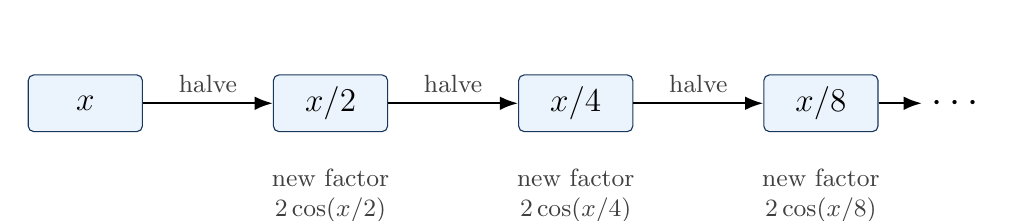
\begin{tikzpicture}[>=Latex, node distance=1.0cm and 1.65cm]
  \tikzset{
    angle/.style={draw=navy,rounded corners=2pt,fill=softblue,
                  minimum width=1.45cm,minimum height=0.72cm,font=\large},
    note/.style={font=\small,align=center,text=black!75}
  }
  \node[angle] (a0) {$x$};
  \node[angle,right=of a0] (a1) {$x/2$};
  \node[angle,right=of a1] (a2) {$x/4$};
  \node[angle,right=of a2] (a3) {$x/8$};
  \node[right=0.55cm of a3,font=\Large] (dots) {$\cdots$};
  \draw[->,thick] (a0) -- node[above,note]{halve} (a1);
  \draw[->,thick] (a1) -- node[above,note]{halve} (a2);
  \draw[->,thick] (a2) -- node[above,note]{halve} (a3);
  \draw[->,thick] (a3) -- (dots);
  \node[note,below=0.34cm of a1] {new factor\\$2\cos(x/2)$};
  \node[note,below=0.34cm of a2] {new factor\\$2\cos(x/4)$};
  \node[note,below=0.34cm of a3] {new factor\\$2\cos(x/8)$};
\end{tikzpicture}

\small Figure 1. Halve the angle; each new angle contributes one new cosine factor.
\end{center}

\section{Background ideas}

\subsection{Angles must be measured in radians}

The proof uses the fundamental limit
\[
  \lim_{u\to 0}\frac{\sin u}{u}=1.
\]
This statement is true in this form only when \(u\) is measured in \emph{radians}.
On a unit circle, an angle of \(u\) radians cuts off an arc of length \(u\). Thus radians connect angles directly to lengths and areas, which is why they naturally appear in limits.

\subsection{What does the product symbol mean?}

The capital Greek letter \(\prod\) means ``multiply a list of terms.'' For example,
\[
  \prod_{k=1}^{4} a_k=a_1a_2a_3a_4.
\]
Therefore,
\[
  \prod_{k=1}^{4}\cos\!\left(\frac{x}{2^k}\right)
  =\cos\!\left(\frac{x}{2}\right)
   \cos\!\left(\frac{x}{4}\right)
   \cos\!\left(\frac{x}{8}\right)
   \cos\!\left(\frac{x}{16}\right).
\]

\begin{definitionBox}[Infinite product]
An infinite product is defined through its \emph{partial products}. If
\[
  P_n=\prod_{k=1}^{n}a_k,
\]
and the numbers \(P_n\) approach a limit \(L\), then we write
\[
  \prod_{k=1}^{\infty}a_k=L.
\]
Infinity is not a final index that we reach. It means that we study what happens as the number of factors \(n\) becomes larger and larger.
\end{definitionBox}

\subsection{The two half-angle identities we need}

For sine, we are given
\[
  \boxed{\sin x=2\sin(x/2)\cos(x/2).}
\]
Later we will also use the cosine half-angle identity
\[
  \boxed{\cos(\theta/2)=\sqrt{\frac{1+\cos\theta}{2}}}
\]
for the small positive angles in this exercise. The positive square root is chosen because all those cosine values are positive.

\section{Repeat the sine half-angle formula}

We first work with only a \emph{finite} number of halvings. This avoids any mystery about infinity.

\subsection{One halving}

The given identity says
\[
  \sin x
  =2\sin\!\left(\frac{x}{2}\right)
     \cos\!\left(\frac{x}{2}\right).
\]

\subsection{Two halvings}

Apply the same identity to \(\sin(x/2)\):
\[
  \sin\!\left(\frac{x}{2}\right)
  =2\sin\!\left(\frac{x}{4}\right)
     \cos\!\left(\frac{x}{4}\right).
\]
Substitute this into the first equation:
\begin{align*}
  \sin x
  &=2\left[
      2\sin\!\left(\frac{x}{4}\right)
       \cos\!\left(\frac{x}{4}\right)
     \right]
     \cos\!\left(\frac{x}{2}\right)\\
  &=2^2\sin\!\left(\frac{x}{4}\right)
     \cos\!\left(\frac{x}{2}\right)
     \cos\!\left(\frac{x}{4}\right).
\end{align*}

\subsection{Three halvings}

Now apply the formula to \(\sin(x/4)\):
\[
  \sin\!\left(\frac{x}{4}\right)
  =2\sin\!\left(\frac{x}{8}\right)
     \cos\!\left(\frac{x}{8}\right).
\]
This gives
\[
  \sin x
  =2^3\sin\!\left(\frac{x}{8}\right)
  \cos\!\left(\frac{x}{2}\right)
  \cos\!\left(\frac{x}{4}\right)
  \cos\!\left(\frac{x}{8}\right).
\]

The pattern is now visible: after \(n\) halvings, there is one small sine term, a factor \(2^n\), and \(n\) cosine factors.

\begin{solutionBox}[Finite repeated-halving identity]
For every positive integer \(n\),
\[
\boxed{\displaystyle
  \sin x
  =2^n\sin\!\left(\frac{x}{2^n}\right)
   \prod_{k=1}^{n}
   \cos\!\left(\frac{x}{2^k}\right).}
\tag{1}
\]
\end{solutionBox}

\subsection{Why formula (1) is always true: a short induction}

A proof by induction is a formal way to confirm that the pattern continues forever.

\textbf{Base case.} For \(n=1\), formula (1) is exactly the given half-angle identity.

\textbf{Induction step.} Suppose formula (1) is true for some \(n\). Then
\[
  \sin\!\left(\frac{x}{2^n}\right)
  =2\sin\!\left(\frac{x}{2^{n+1}}\right)
     \cos\!\left(\frac{x}{2^{n+1}}\right).
\]
Substituting this into (1) adds one factor of \(2\) and one new cosine factor:
\begin{align*}
  \sin x
  &=2^{n+1}\sin\!\left(\frac{x}{2^{n+1}}\right)
    \left(\prod_{k=1}^{n}\cos\!\left(\frac{x}{2^k}\right)\right)
    \cos\!\left(\frac{x}{2^{n+1}}\right)\\
  &=2^{n+1}\sin\!\left(\frac{x}{2^{n+1}}\right)
    \prod_{k=1}^{n+1}\cos\!\left(\frac{x}{2^k}\right).
\end{align*}
So the formula is true for \(n+1\), completing the induction.

\section{Divide by \texorpdfstring{\(x\)}{x} and reveal the small-angle ratio}

Assume first that \(x\ne0\). Divide equation (1) by \(x\):
\[
  \frac{\sin x}{x}
  =\frac{2^n\sin(x/2^n)}{x}
   \prod_{k=1}^{n}\cos\!\left(\frac{x}{2^k}\right).
\]
The first fraction can be rewritten as
\[
  \frac{2^n\sin(x/2^n)}{x}
  =\frac{\sin(x/2^n)}{x/2^n}.
\]
Therefore,
\begin{solutionBox}[The key finite formula]
\[
\boxed{\displaystyle
  \frac{\sin x}{x}
  =\frac{\sin(x/2^n)}{x/2^n}
   \prod_{k=1}^{n}\cos\!\left(\frac{x}{2^k}\right).}
\tag{2}
\]
\end{solutionBox}

This equation separates the problem into two pieces:
\begin{enumerate}
  \item the small-angle factor
  \[
    \frac{\sin(x/2^n)}{x/2^n};
  \]
  \item the partial product
  \[
    P_n=\prod_{k=1}^{n}\cos\!\left(\frac{x}{2^k}\right).
  \]
\end{enumerate}
As \(n\) grows, the angle \(x/2^n\) approaches \(0\). We therefore need to understand \(\sin u/u\) for very small \(u\).

\section{Why \texorpdfstring{\(\sin u/u\)}{sin(u)/u} approaches \texorpdfstring{\(1\)}{1}}

This important limit can be understood geometrically. Take a unit circle and an angle \(u\) with \(0<u<\pi/2\).

\begin{center}
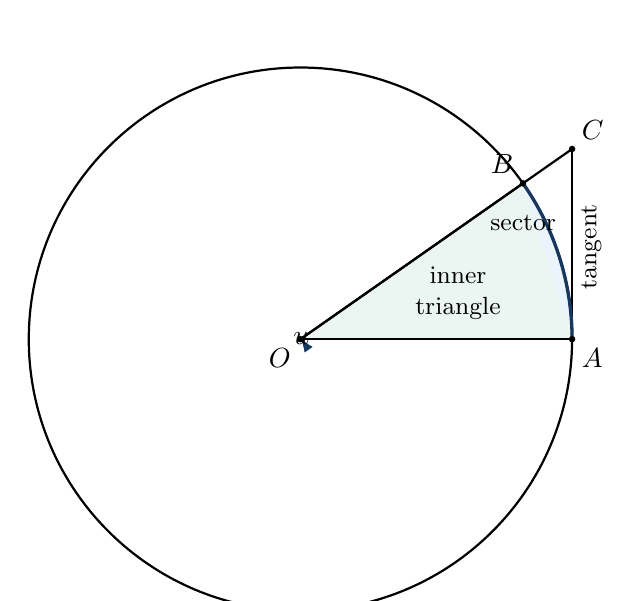
\begin{tikzpicture}[scale=3.45,>=Latex]
  \def\ang{35}
  \coordinate (O) at (0,0);
  \coordinate (A) at (1,0);
  \coordinate (B) at ({cos(\ang)},{sin(\ang)});
  \coordinate (C) at (1,{tan(\ang)});

  \fill[softblue] (O) -- (A) arc[start angle=0,end angle=\ang,radius=1] -- cycle;
  \fill[softgreen,opacity=0.70] (O) -- (B) -- (A) -- cycle;
  \draw[thick] (O) circle (1);
  \draw[thick] (O)--(A);
  \draw[thick] (O)--(B);
  \draw[thick] (O)--(C);
  \draw[thick] (A)--(C);
  \draw[very thick,navy] (A) arc[start angle=0,end angle=\ang,radius=1];
  \draw pic[draw=navy,->,"$u$",angle eccentricity=1.35,angle radius=0.24] {angle=A--O--B};

  \fill (O) circle (0.012) node[below left] {$O$};
  \fill (A) circle (0.012) node[below right] {$A$};
  \fill (B) circle (0.012) node[above left] {$B$};
  \fill (C) circle (0.012) node[above right] {$C$};

  \node[font=\small,align=center] at (0.58,0.17) {inner\\triangle};
  \node[font=\small,align=center] at (0.82,0.43) {sector};
  \node[font=\small,rotate=90] at (1.07,0.34) {tangent};
\end{tikzpicture}

\small Figure 2. The inner triangle lies inside the sector, which lies inside the outer triangle.
\end{center}

For a unit circle:
\begin{itemize}
  \item the inner triangle \(OAB\) has area \(\tfrac12\sin u\);
  \item the circular sector has area \(\tfrac12u\) because \(u\) is in radians;
  \item the outer triangle \(OAC\) has area \(\tfrac12\tan u\).
\end{itemize}
Since the three regions are nested,
\[
  \frac12\sin u<\frac12u<\frac12\tan u.
\]
Multiply by \(2\):
\[
  \sin u<u<\tan u.
\]
The left inequality gives
\[
  \frac{\sin u}{u}<1.
\]
Using \(\tan u=\sin u/\cos u\), the right inequality gives
\[
  u<\frac{\sin u}{\cos u}
  \quad\Longrightarrow\quad
  \cos u<\frac{\sin u}{u}.
\]
Thus
\[
  \cos u<\frac{\sin u}{u}<1.
\]
When \(u\to0\), we have \(\cos u\to1\). The ratio is squeezed between two quantities that both approach \(1\), so
\begin{solutionBox}[Small-angle limit]
\[
  \boxed{\displaystyle \lim_{u\to0}\frac{\sin u}{u}=1.}
\tag{3}
\]
\end{solutionBox}
For negative \(u\), the same conclusion follows because
\[
  \frac{\sin(-u)}{-u}=\frac{\sin u}{u}.
\]

\section{Pass from the finite product to the infinite product}

Let
\[
  u_n=\frac{x}{2^n}.
\]
Because the denominator \(2^n\) grows without bound,
\[
  u_n\longrightarrow0.
\]
By the small-angle limit (3),
\[
  \frac{\sin(x/2^n)}{x/2^n}\longrightarrow1.
\]
Now solve equation (2) for the partial product:
\[
  P_n
  =\prod_{k=1}^{n}\cos\!\left(\frac{x}{2^k}\right)
  =\frac{\sin x/x}{\sin(x/2^n)/(x/2^n)}.
\]
As \(n\to\infty\), the denominator on the right approaches \(1\). Hence
\[
  P_n\longrightarrow\frac{\sin x}{x}.
\]
By the definition of an infinite product,
\begin{solutionBox}[First requested identity]
For \(x\ne0\),
\[
\boxed{\displaystyle
  \frac{\sin x}{x}
  =\prod_{k=1}^{\infty}
   \cos\!\left(\frac{x}{2^k}\right).}
\tag{4}
\]
At \(x=0\), the left side is understood by its continuous extension as \(1\), and every factor on the right is \(\cos0=1\), so the identity remains valid in the extended sense.
\end{solutionBox}

\begin{ideaBox}[What really happened?]
The repeated-halving formula left behind a small sine:
\[
  \sin(x/2^n).
\]
After division by \(x\), this became the ratio
\[
  \frac{\sin(x/2^n)}{x/2^n},
\]
which becomes almost exactly \(1\) when \(n\) is large. The remaining cosine factors therefore carry almost all of the value of \(\sin x/x\).
\end{ideaBox}

\section{Choose \texorpdfstring{\(x=\pi/2\)}{x = pi/2}}

Now substitute \(x=\pi/2\) into (4). The left side is
\[
  \frac{\sin(\pi/2)}{\pi/2}
  =\frac{1}{\pi/2}
  =\frac{2}{\pi}.
\]
The \(k\)-th cosine factor becomes
\[
  \cos\!\left(\frac{\pi/2}{2^k}\right)
  =\cos\!\left(\frac{\pi}{2^{k+1}}\right).
\]
Therefore,
\begin{solutionBox}[Product for \(2/\pi\)]
\[
\boxed{\displaystyle
  \frac{2}{\pi}
  =\prod_{k=1}^{\infty}
   \cos\!\left(\frac{\pi}{2^{k+1}}\right)}
  =\cos\frac{\pi}{4}\,
   \cos\frac{\pi}{8}\,
   \cos\frac{\pi}{16}\cdots .
\tag{5}
\]
\end{solutionBox}

The rest of the exercise is to rewrite these cosine values as nested square roots.

\section{Turn the cosine factors into nested radicals}

\subsection{Derive the cosine half-angle formula}

The double-angle identity
\[
  \cos(2t)=2\cos^2t-1
\]
can be rearranged:
\[
  2\cos^2t=1+\cos(2t),
\]
so
\[
  \cos^2t=\frac{1+\cos(2t)}{2}.
\]
Taking the positive square root for the angles used here gives
\[
  \cos t=\sqrt{\frac{1+\cos(2t)}{2}}.
\]
Writing \(t=\theta/2\), we get
\[
  \boxed{\displaystyle
  \cos\!\left(\frac{\theta}{2}\right)
  =\sqrt{\frac{1+\cos\theta}{2}}.}
\tag{6}
\]

\subsection{Compute the first factor}

Use \(\theta=\pi/2\):
\begin{align*}
  \cos\frac{\pi}{4}
  &=\sqrt{\frac{1+\cos(\pi/2)}{2}}\\
  &=\sqrt{\frac{1+0}{2}}\\
  &=\frac{\sqrt2}{2}.
\end{align*}

\subsection{Compute the second factor}

Use \(\theta=\pi/4\):
\begin{align*}
  \cos\frac{\pi}{8}
  &=\sqrt{\frac{1+\cos(\pi/4)}{2}}\\
  &=\sqrt{\frac{1+\sqrt2/2}{2}}\\
  &=\sqrt{\frac{2+\sqrt2}{4}}\\
  &=\frac{\sqrt{2+\sqrt2}}{2}.
\end{align*}

\needspace{18\baselineskip}
\subsection{Compute the third factor}

Use \(\theta=\pi/8\):
\begin{align*}
  \cos\frac{\pi}{16}
  &=\sqrt{\frac{1+\cos(\pi/8)}{2}}\\
  &=\sqrt{\frac{1+\frac12\sqrt{2+\sqrt2}}{2}}\\
  &=\frac{\sqrt{2+\sqrt{2+\sqrt2}}}{2}.
\end{align*}

Each new radical is obtained by placing the previous radical after another \(2+\) and then taking a square root.

\begin{center}
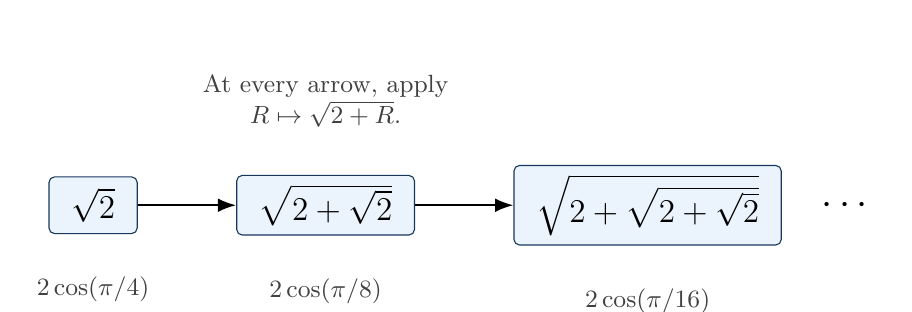
\begin{tikzpicture}[>=Latex,node distance=1.25cm]
  \tikzset{
    rad/.style={draw=navy,fill=softblue,rounded corners=2pt,
                minimum height=0.72cm,inner xsep=8pt,font=\large},
    lab/.style={font=\small,text=black!75,align=center}
  }
  \node[rad] (r1) {$\sqrt2$};
  \node[rad,right=of r1] (r2) {$\sqrt{2+\sqrt2}$};
  \node[rad,right=of r2] (r3) {$\sqrt{2+\sqrt{2+\sqrt2}}$};
  \draw[->,thick] (r1.east)--(r2.west);
  \draw[->,thick] (r2.east)--(r3.west);
  \node[right=0.38cm of r3,font=\Large] {$\cdots$};
  \node[lab,above=0.48cm of r2] {At every arrow, apply\\$R\mapsto\sqrt{2+R}$.};
  \node[below=0.42cm of r1,lab] {$2\cos(\pi/4)$};
  \node[below=0.42cm of r2,lab] {$2\cos(\pi/8)$};
  \node[below=0.42cm of r3,lab] {$2\cos(\pi/16)$};
\end{tikzpicture}

\small Figure 3. The nested radicals follow the same repeated-halving pattern as the angles.
\end{center}

\subsection{A clean recursive description}

Define
\[
  R_1=\sqrt2,
  \qquad
  R_{n+1}=\sqrt{2+R_n}.
\]
Then
\[
  R_n=2\cos\!\left(\frac{\pi}{2^{n+1}}\right).
\]
To see why, check the first value:
\[
  R_1=\sqrt2=2\cos\frac{\pi}{4}.
\]
If \(R_n=2\cos\theta\), then
\begin{align*}
  R_{n+1}
  &=\sqrt{2+2\cos\theta}\\
  &=\sqrt{4\cos^2(\theta/2)}\\
  &=2\cos\frac{\theta}{2},
\end{align*}
where the last cosine is positive. Thus one radical step corresponds exactly to halving the angle.

Substituting the radical forms into equation (5) gives the requested result.

\begin{solutionBox}[Second requested identity: Vi\`ete's formula]
\[
\boxed{\displaystyle
\frac{2}{\pi}
=\frac{\sqrt2}{2}\cdot
 \frac{\sqrt{2+\sqrt2}}{2}\cdot
 \frac{\sqrt{2+\sqrt{2+\sqrt2}}}{2}\cdots .}
\tag{7}
\]
This is commonly called Vi\`ete's product for \(2/\pi\).
\end{solutionBox}

\section{A numerical check}

An infinite identity becomes easier to trust when its first few partial products move toward the claimed value. Let
\[
  V_n=\prod_{k=1}^{n}\cos\!\left(\frac{\pi}{2^{k+1}}\right).
\]
The target value is
\[
  \frac{2}{\pi}\approx0.6366197724.
\]

\begin{center}
\renewcommand{\arraystretch}{1.18}
\begin{tabular}{>{\centering\arraybackslash}p{0.10\textwidth}
                >{\centering\arraybackslash}p{0.27\textwidth}
                >{\centering\arraybackslash}p{0.25\textwidth}}
\toprule
\(n\) & New factor & Partial product \(V_n\) \\
\midrule
1 & \(\cos(\pi/4)\)  & \(0.7071067812\) \\
2 & \(\cos(\pi/8)\)  & \(0.6532814824\) \\
3 & \(\cos(\pi/16)\) & \(0.6407288619\) \\
4 & \(\cos(\pi/32)\) & \(0.6376435773\) \\
5 & \(\cos(\pi/64)\) & \(0.6368755077\) \\
6 & \(\cos(\pi/128)\)& \(0.6366836927\) \\
\bottomrule
\end{tabular}
\end{center}

The values decrease toward \(0.6366197724\), exactly as the formula predicts. Later factors are very close to \(1\), but multiplying many of them still makes a small correction.

\section{A concise proof suitable for a homework submission}

The following is a compact version of the argument after you understand all the steps.

\begin{solutionBox}[Complete proof]
Repeated use of
\[
  \sin t=2\sin(t/2)\cos(t/2)
\]
gives, for every \(n\ge1\),
\[
  \sin x
  =2^n\sin\!\left(\frac{x}{2^n}\right)
   \prod_{k=1}^{n}\cos\!\left(\frac{x}{2^k}\right).
\]
For \(x\ne0\), division by \(x\) yields
\[
  \frac{\sin x}{x}
  =\frac{\sin(x/2^n)}{x/2^n}
   \prod_{k=1}^{n}\cos\!\left(\frac{x}{2^k}\right).
\]
Since \(x/2^n\to0\) and \(\lim_{u\to0}\sin u/u=1\), taking \(n\to\infty\) gives
\[
  \frac{\sin x}{x}
  =\prod_{k=1}^{\infty}\cos\!\left(\frac{x}{2^k}\right).
\]
Now set \(x=\pi/2\). Since \(\sin(\pi/2)=1\),
\[
  \frac{2}{\pi}
  =\cos\frac{\pi}{4}\cos\frac{\pi}{8}
   \cos\frac{\pi}{16}\cdots .
\]
Using
\[
  \cos(\theta/2)=\sqrt{\frac{1+\cos\theta}{2}},
\]
we obtain
\[
  \cos\frac{\pi}{4}=\frac{\sqrt2}{2},
\]
\[
  \cos\frac{\pi}{8}=\frac{\sqrt{2+\sqrt2}}{2},
\]
and
\[
  \cos\frac{\pi}{16}
  =\frac{\sqrt{2+\sqrt{2+\sqrt2}}}{2},
\]
with the same pattern continuing. Therefore,
\[
  \frac{2}{\pi}
  =\frac{\sqrt2}{2}\cdot
   \frac{\sqrt{2+\sqrt2}}{2}\cdot
   \frac{\sqrt{2+\sqrt{2+\sqrt2}}}{2}\cdots .
\]
\end{solutionBox}

\section{Common mistakes and how to avoid them}

\begin{warningBox}[Mistake 1: losing powers of \(2\)]
Every halving introduces a factor of \(2\). After \(n\) halvings, the coefficient is \(2^n\), not merely \(2n\) or \(2\).
\end{warningBox}

\begin{warningBox}[Mistake 2: an index shift]
After setting \(x=\pi/2\),
\[
  \frac{x}{2^k}=\frac{\pi}{2^{k+1}}.
\]
Thus the first factor is \(\cos(\pi/4)\), not \(\cos(\pi/2)\).
\end{warningBox}

\begin{warningBox}[Mistake 3: treating infinity as a final step]
We never ``plug in \(n=\infty\).'' We form the finite partial products \(P_n\) and then take the limit as \(n\to\infty\).
\end{warningBox}

\begin{warningBox}[Mistake 4: choosing the wrong square root]
From \(z^2=A\), one normally has \(z=\pm\sqrt A\). Here all angles \(\pi/4,\pi/8,\ldots\) lie between \(0\) and \(\pi/2\), where cosine is positive. Therefore we use the positive root.
\end{warningBox}

\begin{warningBox}[Mistake 5: using degrees in the small-angle limit]
The limit \(\sin u/u\to1\) requires radian measure. In degrees, a conversion factor would appear.
\end{warningBox}

\section{Check your understanding}

Try these before reading the answers.

\begin{enumerate}
  \item Write the repeated-halving identity after exactly four halvings.
  \item Explain in one sentence why \(x/2^n\to0\).
  \item What is the fourth cosine factor after setting \(x=\pi/2\)?
  \item Let \(R_1=\sqrt2\) and \(R_{n+1}=\sqrt{2+R_n}\). Write \(R_4\).
  \item Why is the positive square root used in the cosine half-angle formula here?
\end{enumerate}

\needspace{10\baselineskip}
\textbf{Answers.}
\begin{enumerate}
  \item
  \[
    \sin x=2^4\sin\frac{x}{16}
    \cos\frac{x}{2}\cos\frac{x}{4}
    \cos\frac{x}{8}\cos\frac{x}{16}.
  \]
  \item The numerator \(x\) stays fixed while the positive denominator \(2^n\) grows without bound.
  \item \(\cos(\pi/32)\), because the \(k\)-th factor is \(\cos(\pi/2^{k+1})\).
  \item
  \[
    R_4=\sqrt{2+\sqrt{2+\sqrt{2+\sqrt2}}}.
  \]
  \item All relevant angles lie in the first quadrant, where cosine is positive.
\end{enumerate}

\section{Final summary}

The proof has one repeating mechanism and one limiting step:
\[
\boxed{
\begin{array}{c}
\text{halve the angle repeatedly}\\[0.2em]
\Downarrow\\[0.2em]
\sin x=2^n\sin(x/2^n)
\displaystyle\prod_{k=1}^{n}\cos(x/2^k)\\[0.4em]
\Downarrow\ \text{divide by }x\\[0.2em]
\displaystyle
\frac{\sin x}{x}
=\frac{\sin(x/2^n)}{x/2^n}
\prod_{k=1}^{n}\cos(x/2^k)\\[0.4em]
\Downarrow\ n\to\infty,
\quad \frac{\sin u}{u}\to1\\[0.2em]
\displaystyle
\frac{\sin x}{x}
=\prod_{k=1}^{\infty}\cos(x/2^k).
\end{array}}
\]
Choosing \(x=\pi/2\) changes the left side into \(2/\pi\). Repeated use of the cosine half-angle identity changes the factors on the right into nested radicals. That is Vi\`ete's elegant product.

\end{document}
